\section{Concepts}
\label{sec:concepts}

\subsection{XText Projects}
\label{sec:xtext-projects}

Each project containing CamilleX constructs must be set to be XText project.  An XText project has an associated XContext and XMachine builders that can compile CamilleX source files into Rodin files as they are changed.  The builders can be turn off via the preferences, either workspace-wise or project-wise (see Figure~\ref{fig:XContextPreference}.
\begin{figure}[!htbp]
  \centering
  \ifplastex
  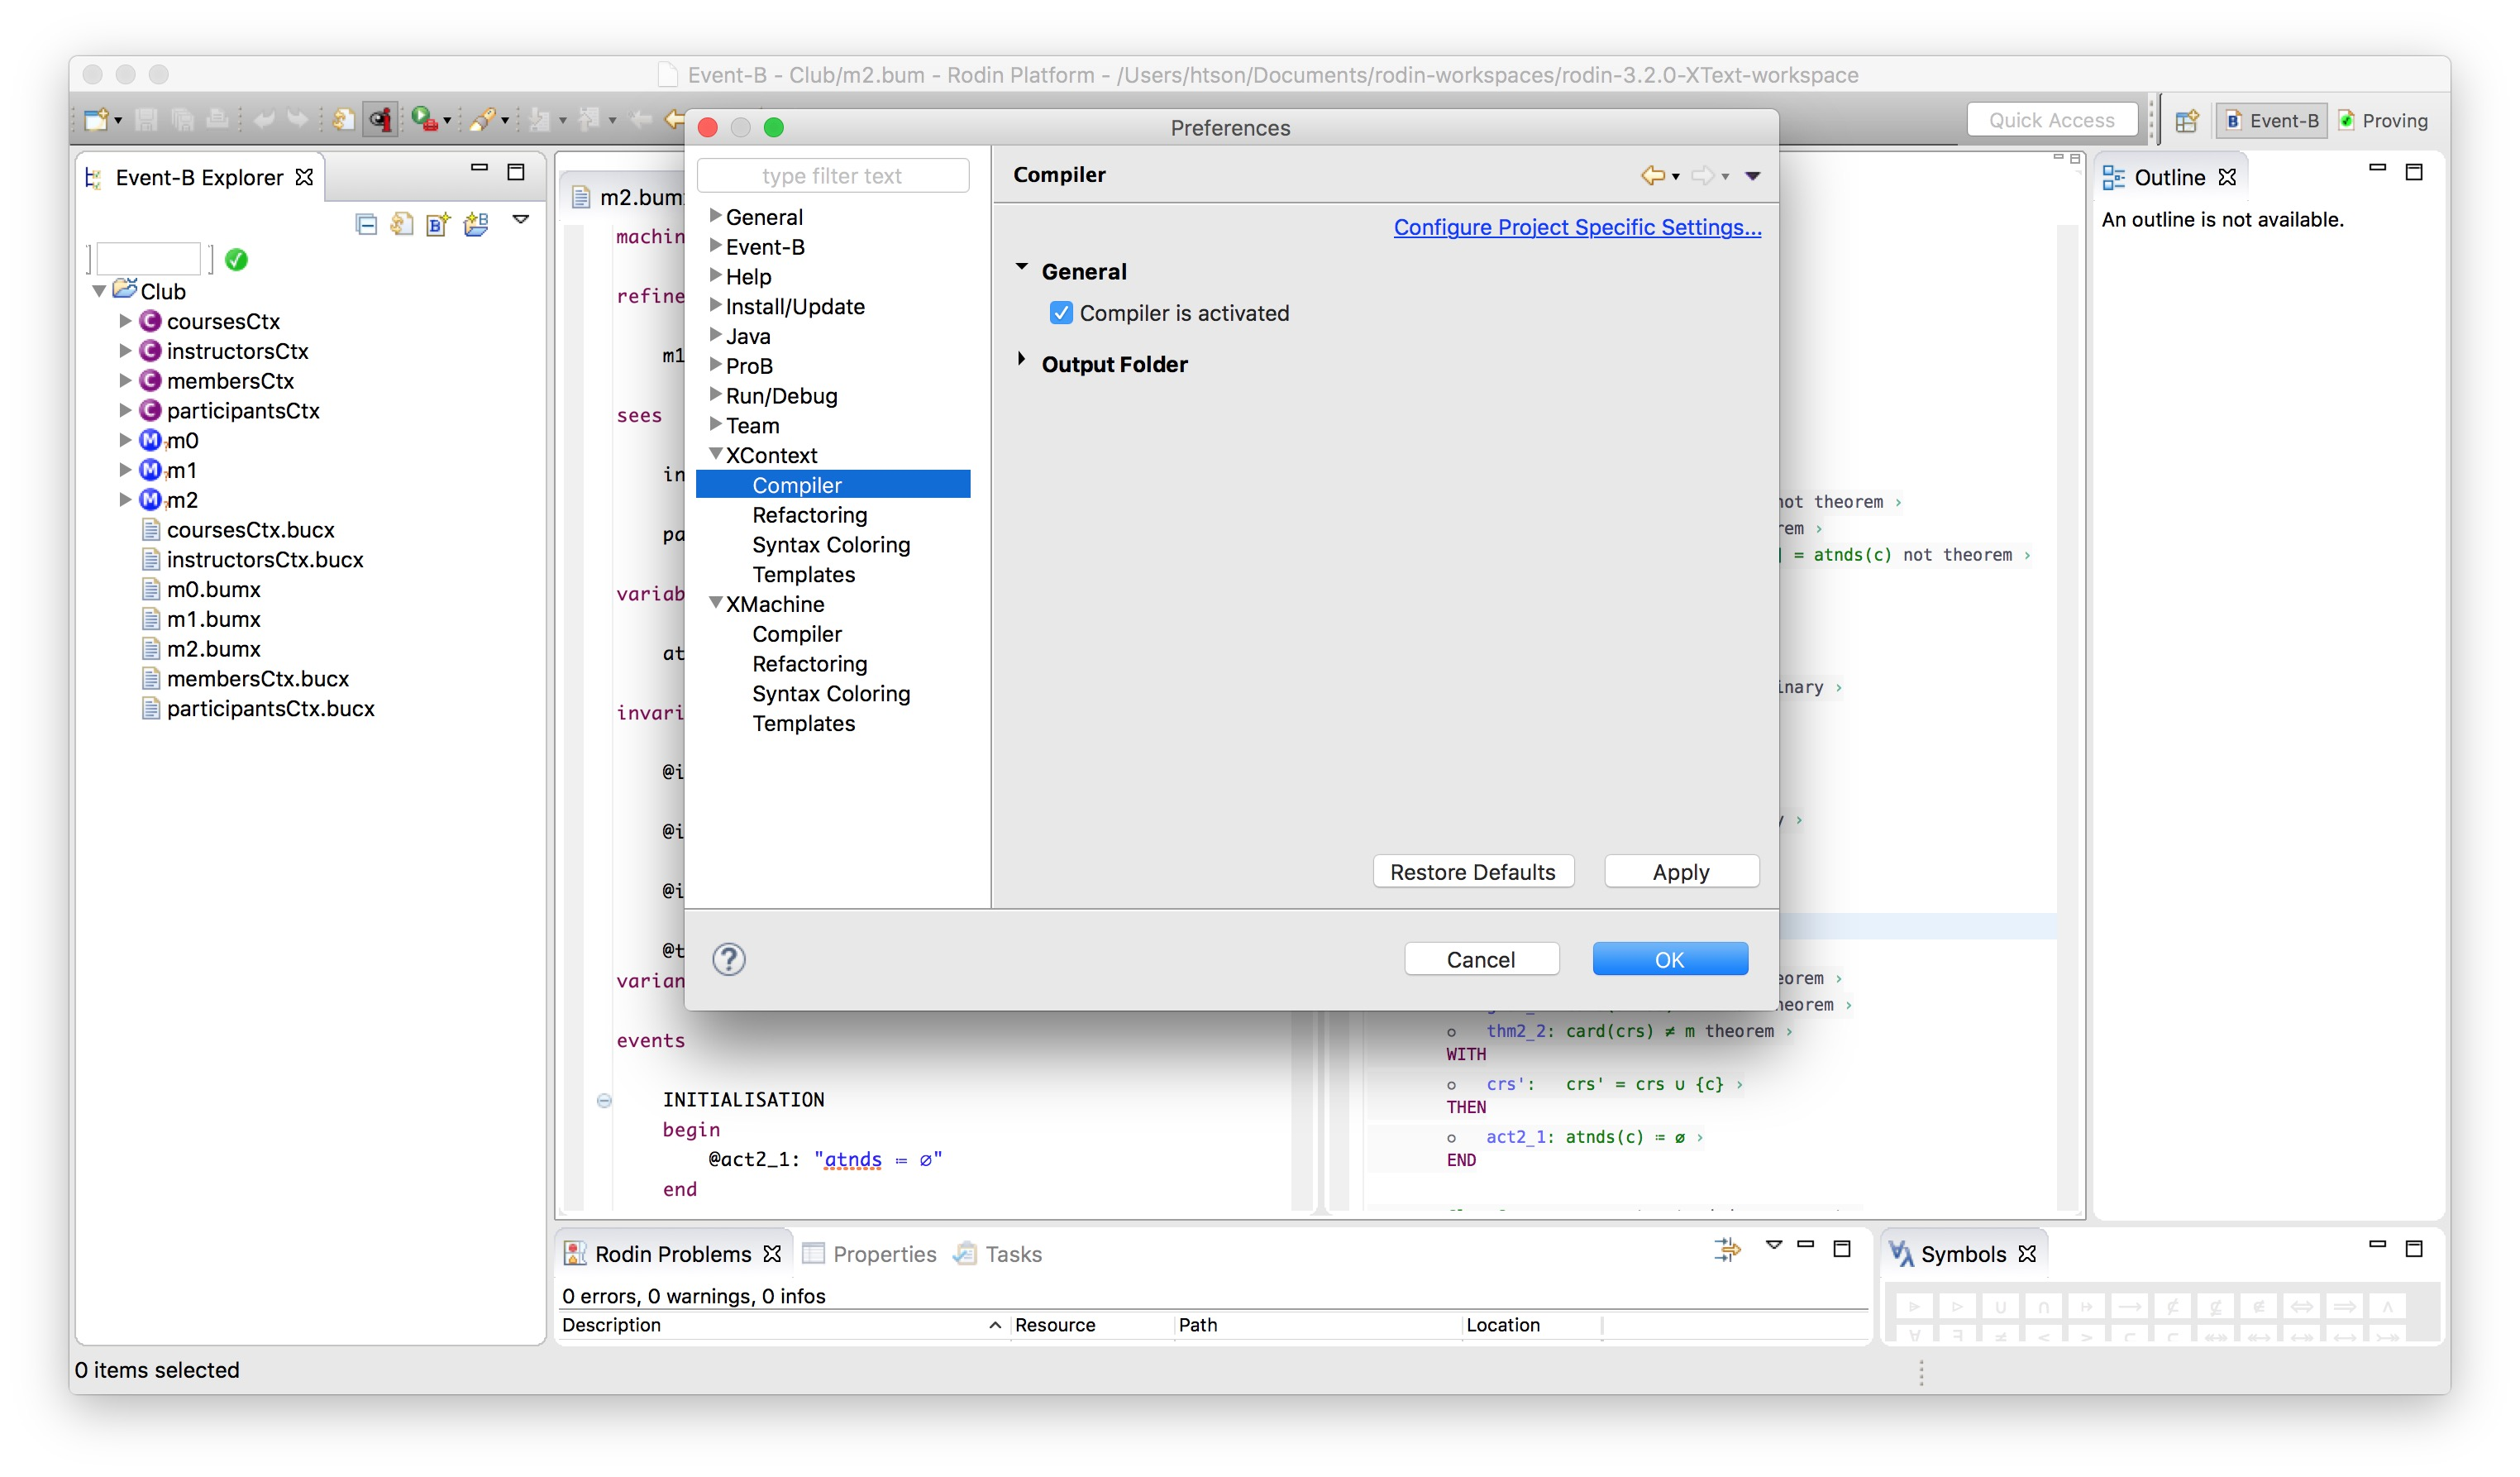
\includegraphics[width=512]{figures/XContextPreference}
  \else
  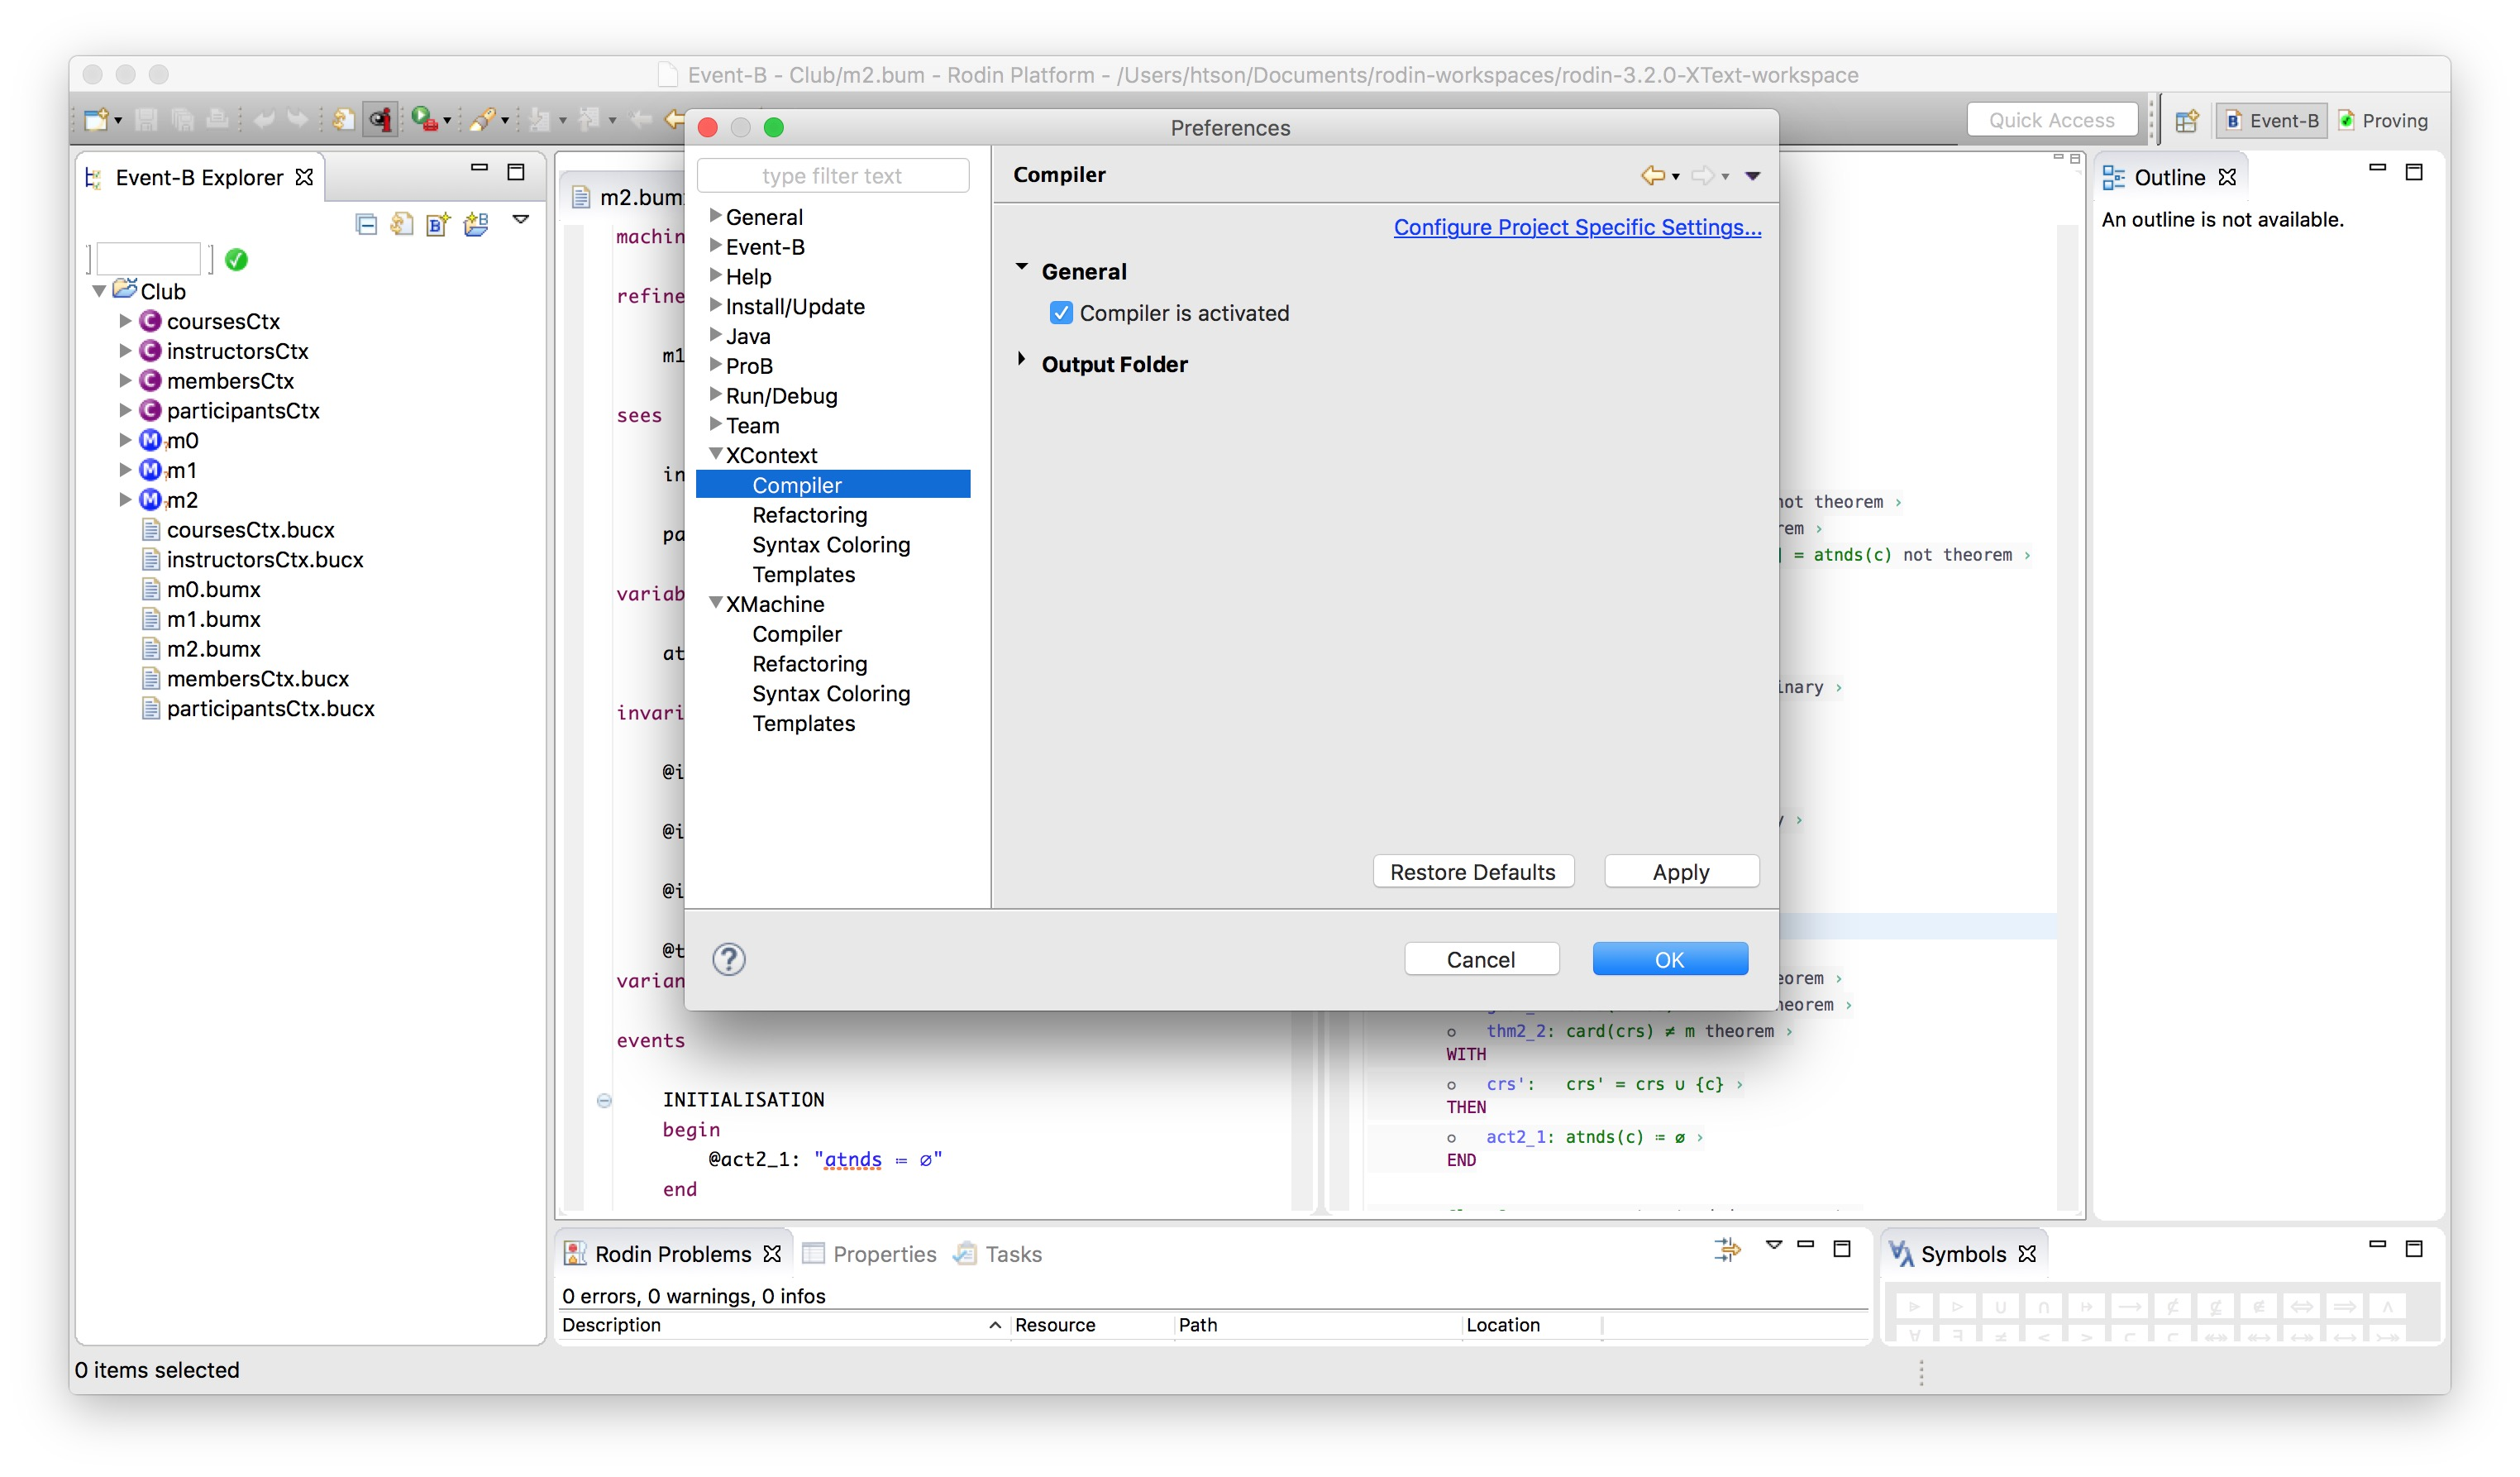
\includegraphics[width=0.9\textwidth]{figures/XContextPreference}
  \fi
  \caption{XContext Preference}
  \label{fig:XContextPreference}
\end{figure}

The XText projects must be organised such that all CamilleX constructs has the project as the source container.

\subsection{CamilleX Builders}
\label{sec:xevent-b-builders}
The CamilleX Builders, i.e., XContext builder and XMachine builder, build CamilleX constructs, i.e., XContext and XMachine using their own compiler.  If they are enabled, the CamilleX builders are run everytime an individual CamilleX file is saved.  Problems detected by the CamilleX builders are classified as either warnings or errors.  Compile-time errors are always reported as errors by the CamilleX buiders and in the presence of errors, no new Rodin files are created or updated, i.e., the CamilleX builders do not produce any new Rodin file content. In the case of machine inclusion and event synchronisation, a flattened machine is generated which includes data from the included machine and the synchronised events, which can be renamed if prefixing is applied.

\subsection{Content Assist}
\label{sec:content-assist}
Content assist are available for typesetting keywords and Event-B mathematical symbols. The short-cut for invoking content assist is \texttt{Ctrl+Space}.  Figure~\ref{fig:KeywordContentAssist} shows an example for content assist with keywords.
\begin{figure}[!htbp]
  \centering
  \ifplastex
  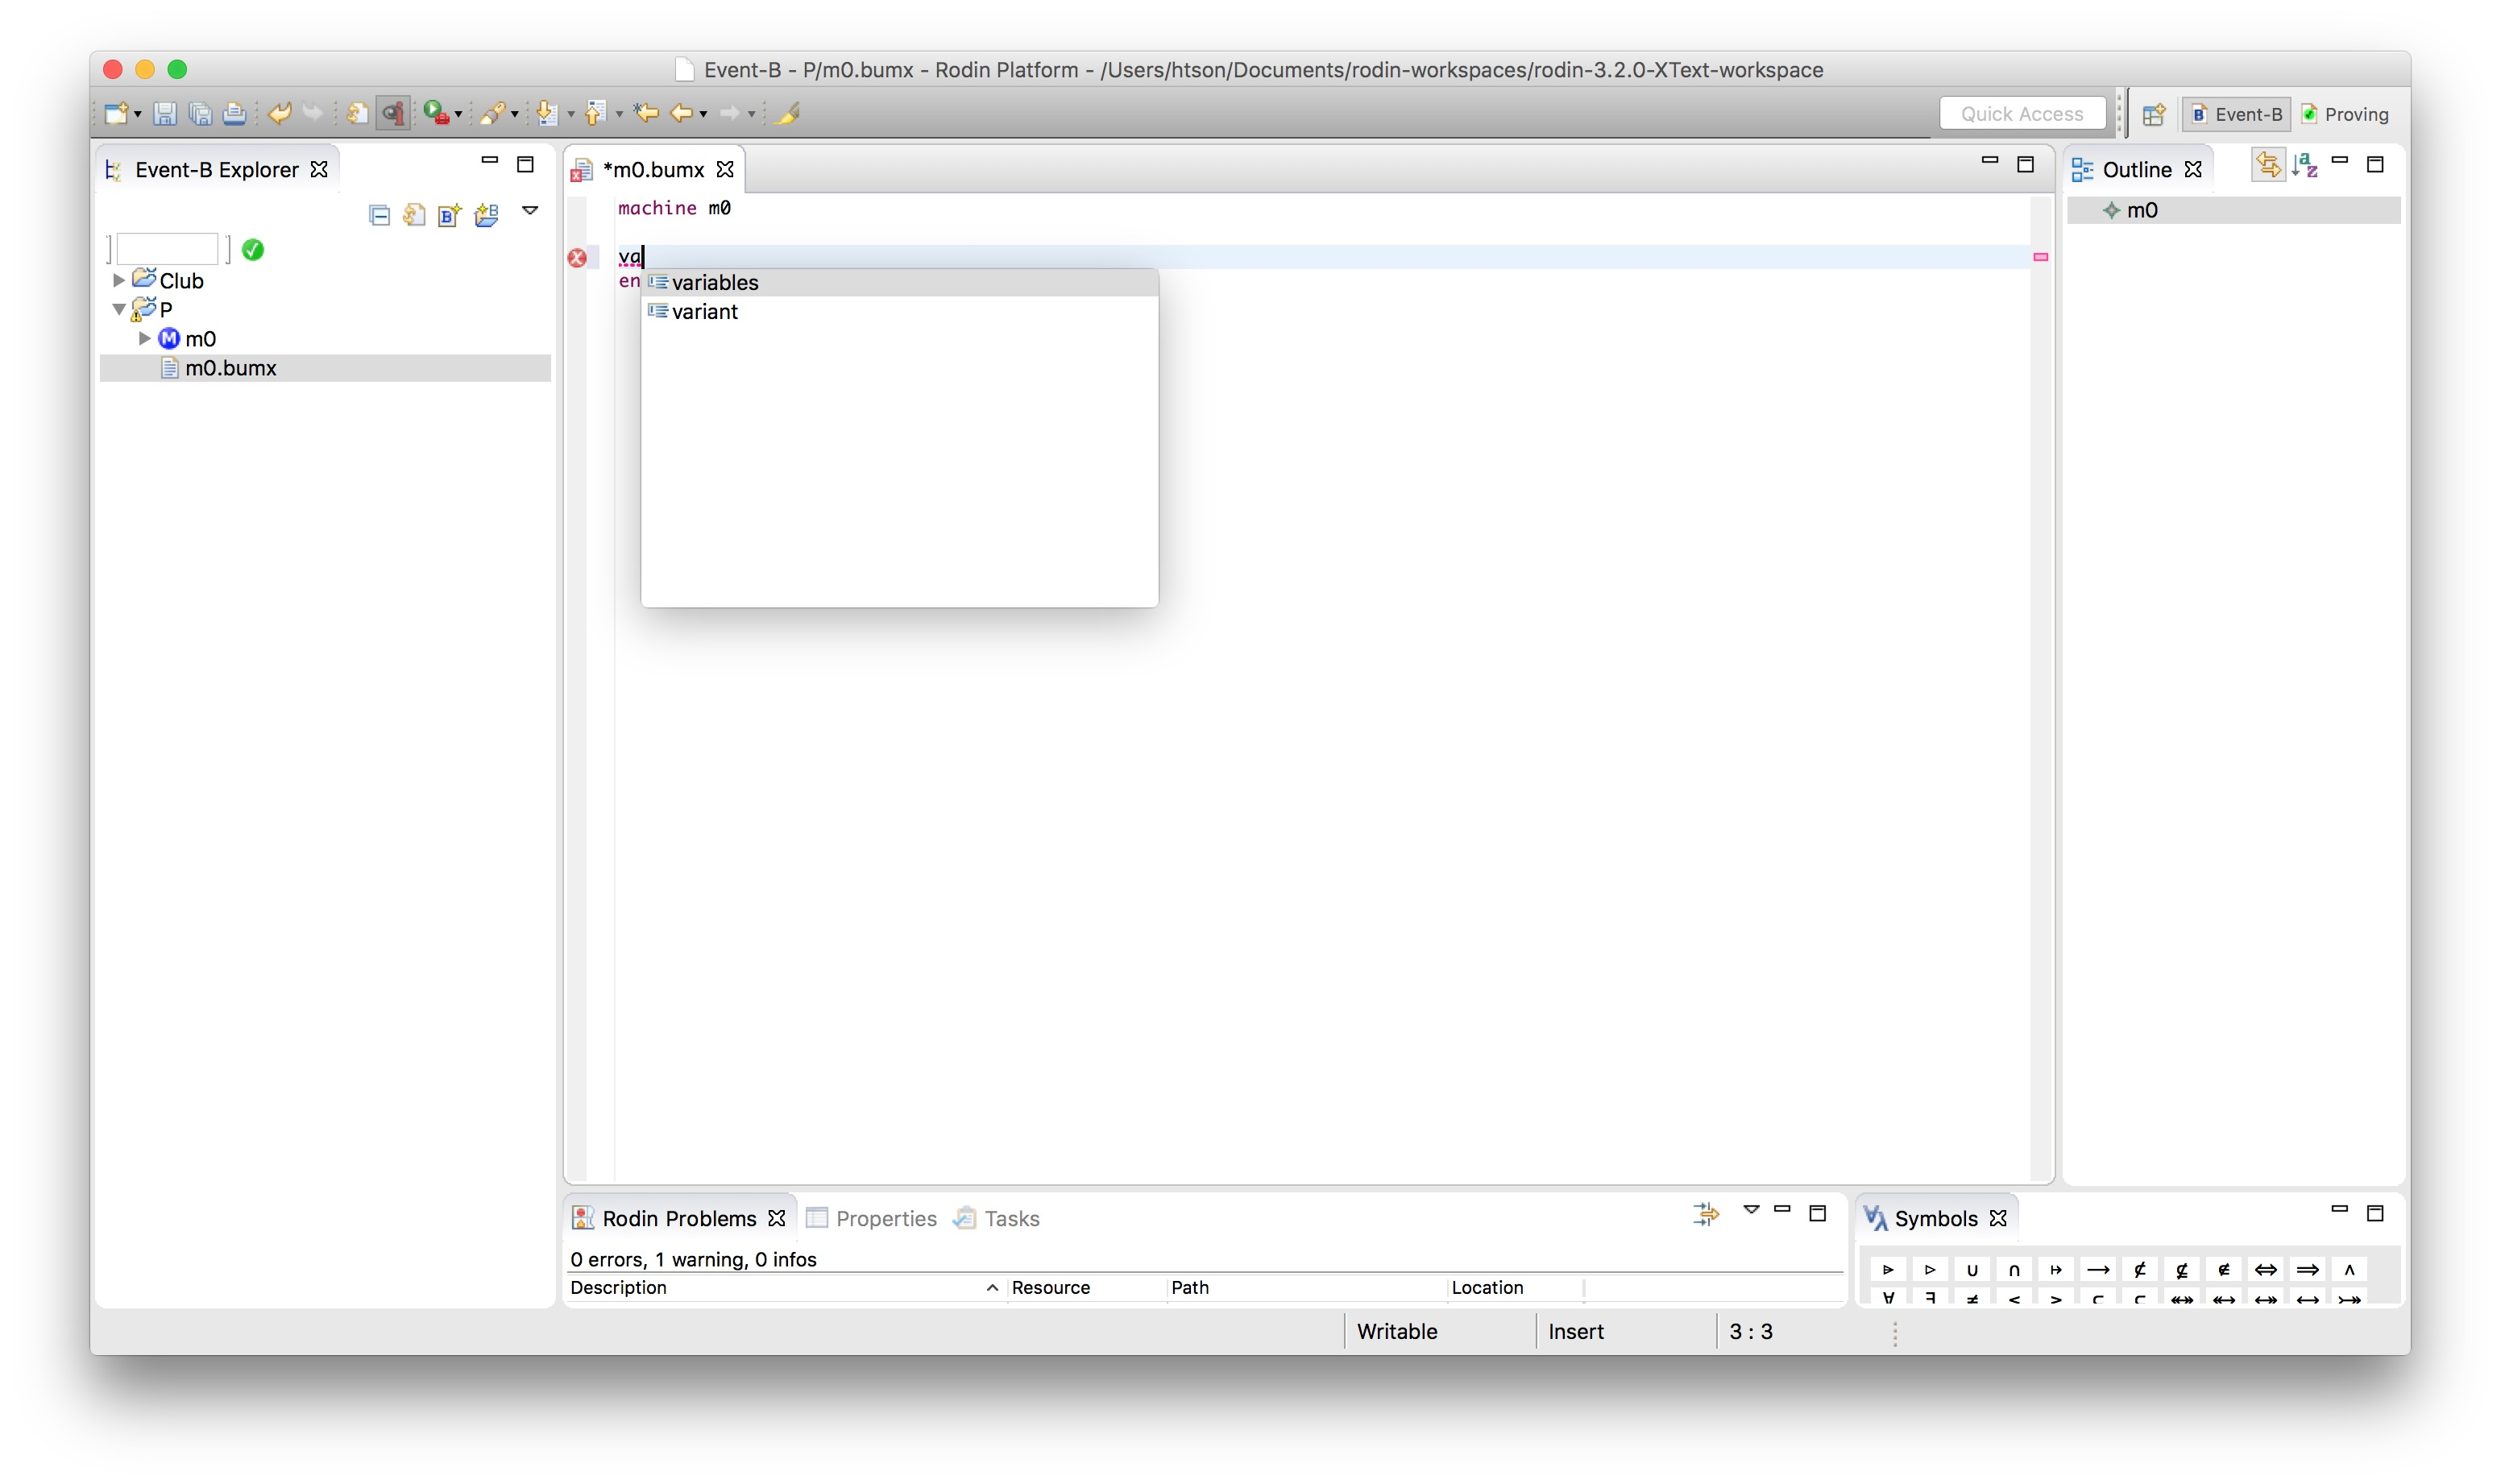
\includegraphics[width=512]{figures/KeywordContentAssist}
  \else
  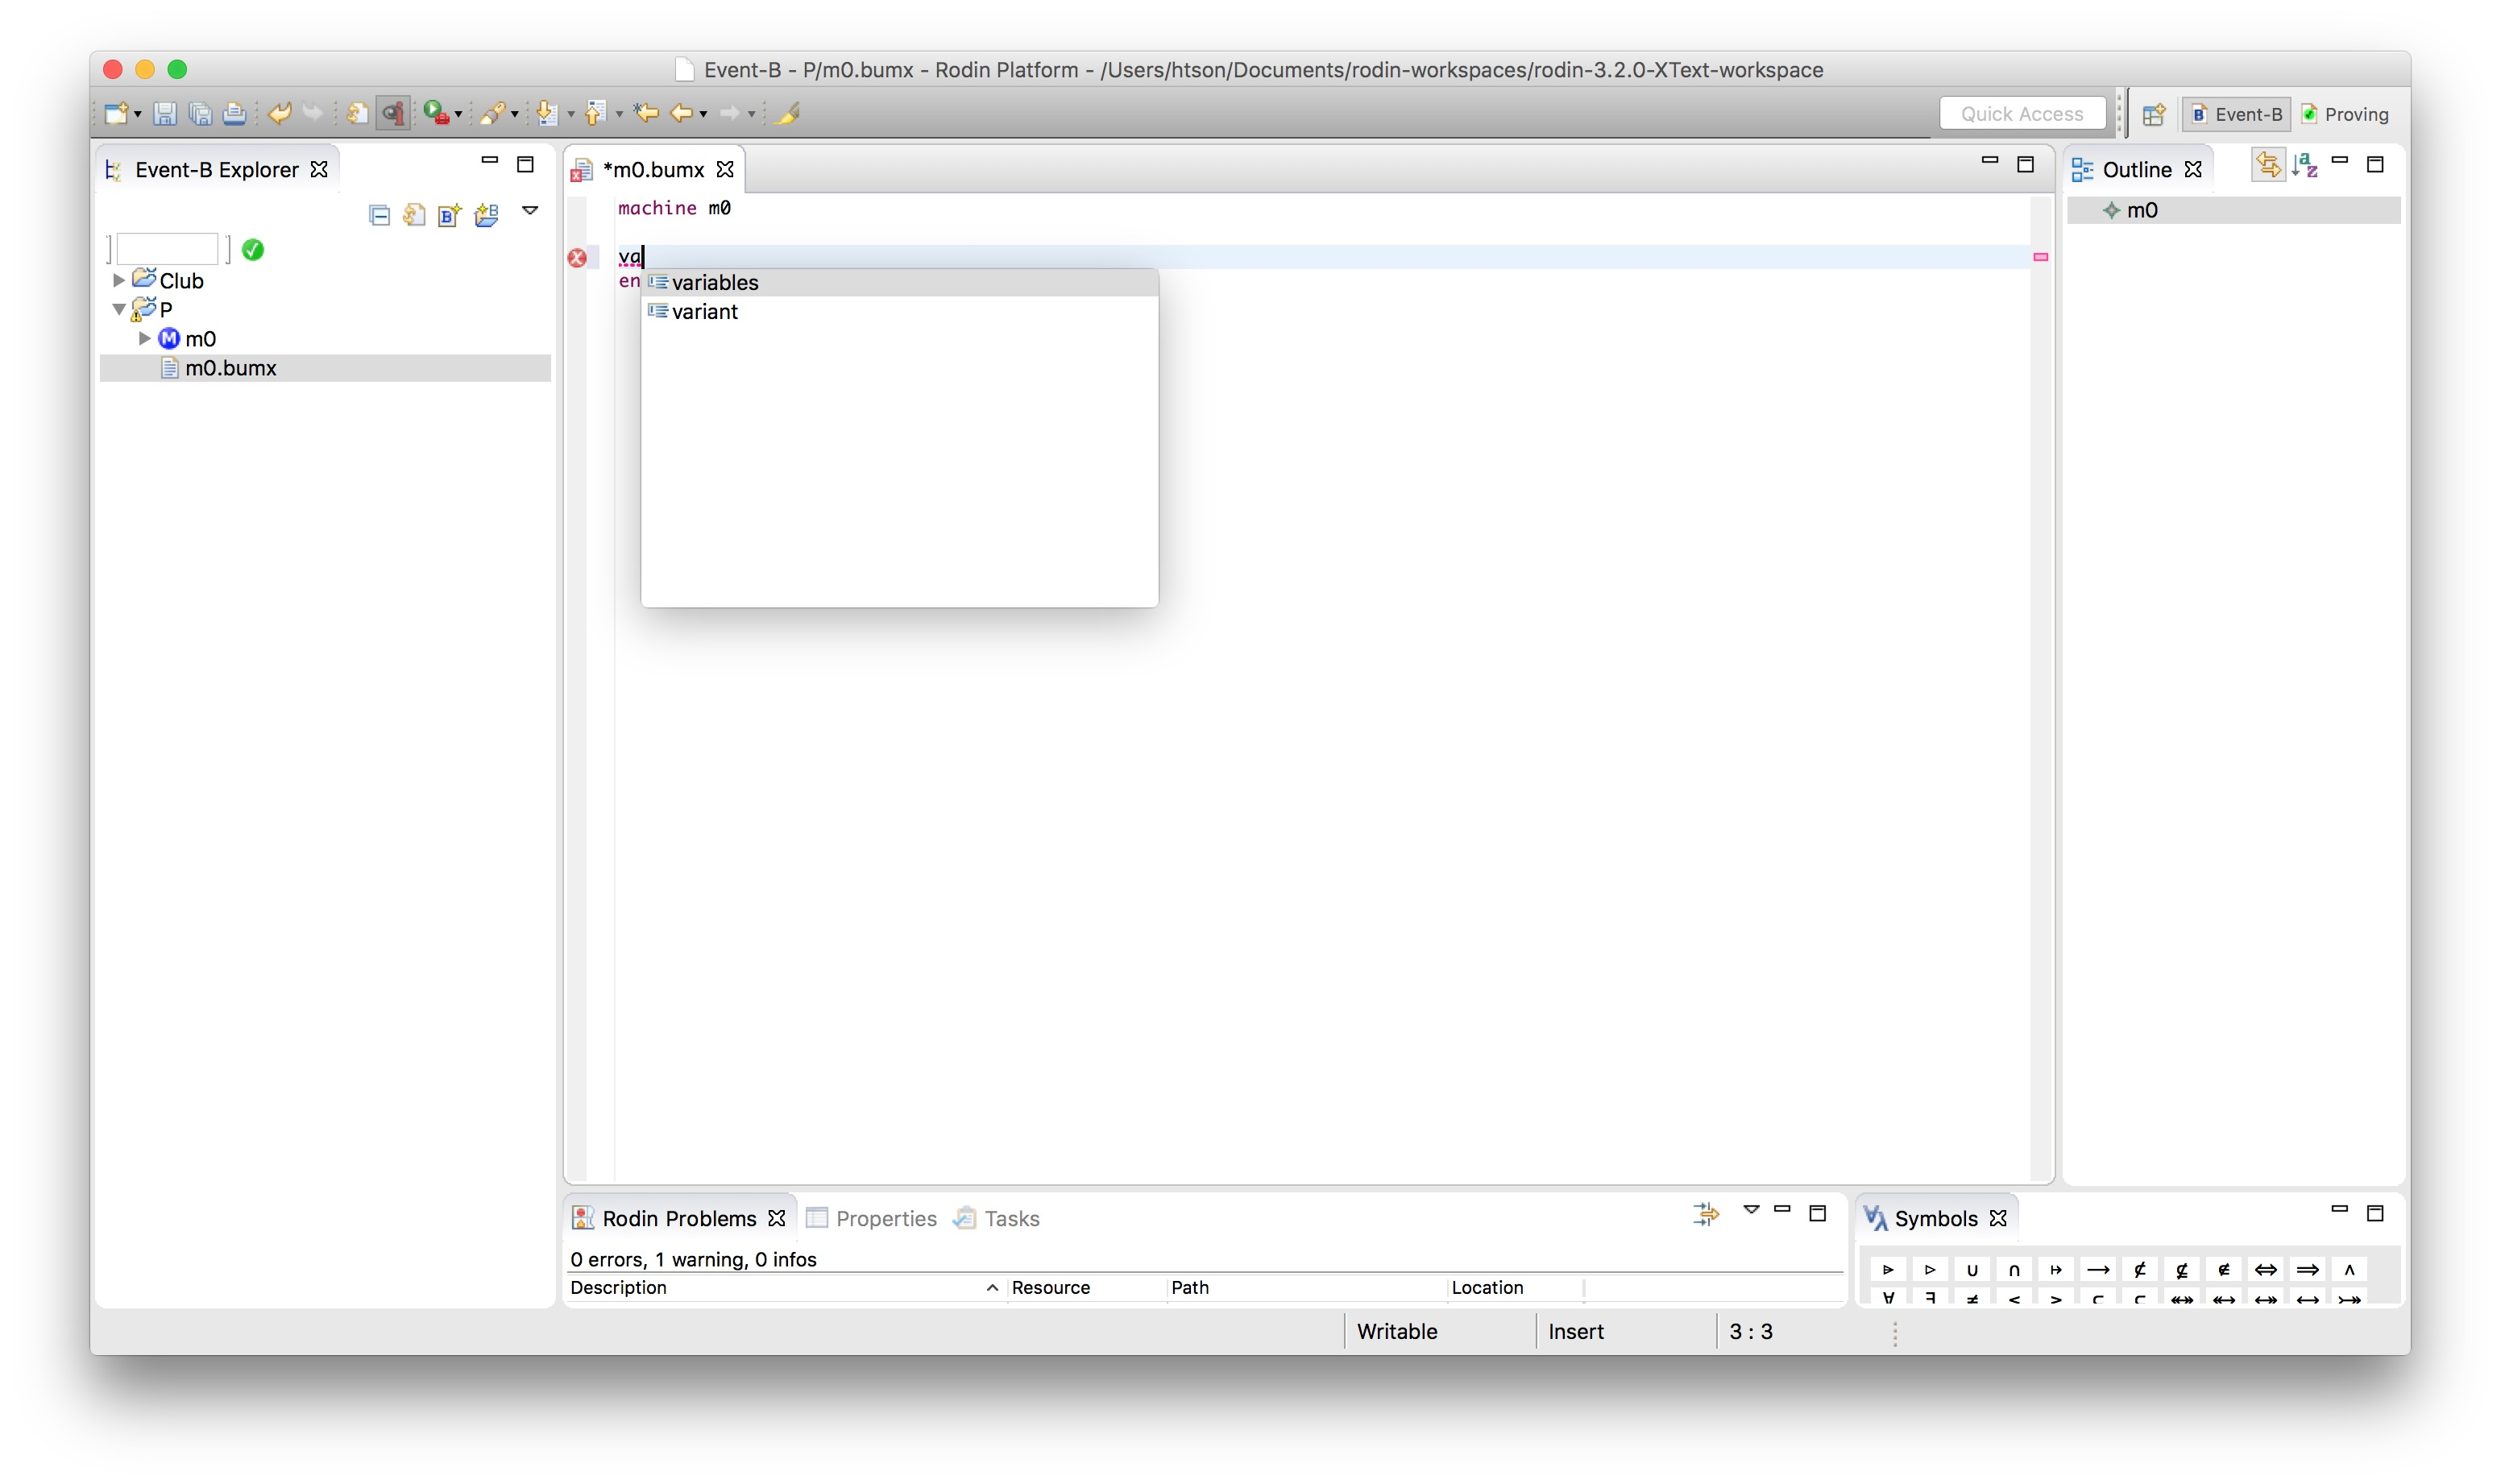
\includegraphics[width=0.9\textwidth]{figures/KeywordContentAssist}
  \fi
  \caption{Keyword Content Assist}
  \label{fig:KeywordContentAssist}
\end{figure}
For Event-B mathematical symbols, the key combination is defined by the Rodin Keyboard plug-in.


%%% Local Variables:
%%% mode: latex
%%% TeX-master: "user_manual"
%%% End:
